\documentclass{article}

\usepackage[utf8]{inputenc}

\usepackage{nicefrac}
\usepackage{amssymb, amsmath, amsfonts}
\usepackage{amsthm}
\usepackage{tikz}
\usetikzlibrary{matrix,shapes,arrows, calc, intersections}
\usetikzlibrary{decorations.markings}
\usepackage{pgfplots}
\usepackage{tkz-euclide}
\usetkzobj{angles} % important you want to use angles
\usepgfplotslibrary{groupplots}
\usepackage[a4paper, margin=1in]{geometry}

\newtheorem{proposition}{Proposition}
\newtheorem{theorem}{Theorem}
\newtheorem{definition}{Definition}
\newtheorem{lemma}{Lemma}
\newtheorem{conjecture}{Conjecture}
\newtheorem{corollary}{Corollary}
\newtheorem{remark}{Remark}
\newtheorem{assumption}{Assumption}

\newlength\figureheight
\newlength\figurewidth
\setlength\figureheight{12cm}
\setlength\figurewidth{14cm}

\newcommand{\tikzdir}[1]{tikz/#1.tikz}
\newcommand{\inputtikz}[1]{\input{\tikzdir{#1}}}

\DeclareMathOperator*{\argmin}{arg\; min}     % argmin
\DeclareMathOperator*{\argmax}{arg\; max}     % argmax
\DeclareMathOperator*{\tr}{tr}     % trace
\DeclareMathOperator{\Cov}{Cov}
\DeclareMathOperator{\logdet}{log\;det}

\title{EE8087 Living with Mathematics\\Tutorial 5: Astronomy}
\date{}
\begin{document} \maketitle
\begin{enumerate}
\item Suppose Earth is a perfect sphere with radius $6371$km. A sailor is standing on the top of a mast $10$m above sea level. Can she see a light tower $30$km away and $20$m above sea level?


\item Suppose 2 people standing at point $A$ and $B$ with the same longitude. The latitude difference between $A$ and $B$ is $\angle AOB = 150^\circ$. Person $A$ find the moon is on the horizon while person $B$ measures that the moon is $\alpha = 60.83^\circ$ away from the zenith. Suppose Earth is a perfect sphere with radius 1. Compute the distance from the center of Earth to the Moon $OM$.
\begin{figure}[ht]
  \centering
  \begin{tikzpicture}
    \tkzDefPoint[label=135:$A$](0,1){A}
    \tkzDefPoint[label=180:$O$](0,0){O}
    \tkzDefPoint[label=225:$B$](-60:1){B}
    \tkzDefPoint(10,1){M}
    \tkzDrawCircle[R](O,1 cm)
    \tkzDrawLine[add=0 and .3](O,A) 
    \tkzDrawLine[add=0 and .3](O,B) 
    \tkzDrawSegments(O,M A,M B,M)
    \tkzDrawPoints(A,B,O,M)
    \tkzLabelPoints(M)
    \draw (-60:1.2) arc (-60:11.11:0.2) node [midway, right] {$\alpha$};
    \draw (0,1.15)--(0.15,1.15)--(0.15,1);
  \end{tikzpicture}
\end{figure}
\item A type Ia supernova is known to have a typical absolute magnitude of $M = -19.3$, with little variation. Suppose we observe a type Ia supernova in a distant galaxy with apparent magnitude $m=12$. What is the distance between us and the supernova?
\item  The orbit of the Moon is an ellipse with eccentricity $0.0549$. Suppose it can be written in the standard form
  \begin{align*}
    \frac{x^2}{a^2}+\frac{y^2}{b^2} = 1,
  \end{align*}
   with Earth on the right focus. Suppose Moon rotates in counterclockwise fashion. If the orbital period of the moon is 27.32 days, how long does it take the moon to travel from $A$ to $B$? and how long does it take to travel from $B$ to $A$?

  \begin{figure}[ht]
    \centering
    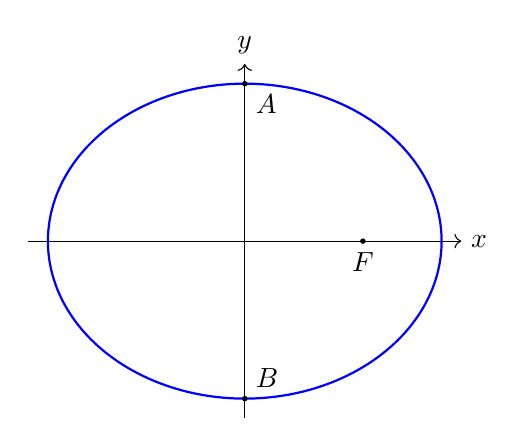
\begin{tikzpicture}[scale=0.5]
      \draw[->] (-5.5,0) -- (5.5,0) node[right] {$x$};
      \draw[->] (0,-4.5) -- (0,4.5) node[above] {$y$};
      \draw[domain=0:2*pi, samples=200,smooth,variable=\t,blue,thick] plot ({5*cos(\t r)},{4*sin(\t r)});
      \node [inner sep=0, outer sep=0, label=270:$F$] (F) at (3,0) {}; 
      \fill [black] (F) circle (2pt); 

      \node [inner sep=0, outer sep=0, label=-45:$A$] (A) at (0,4) {}; 
      \fill [black] (A) circle (2pt); 

      \node [inner sep=0, outer sep=0, label=45:$B$] (B) at (0,-4) {}; 
      \fill [black] (B) circle (2pt); 
    \end{tikzpicture}
  \end{figure}

\item The orbit of Halley comet has an eccentricity of $0.96714$ and its orbital period is 75.32 year. Compute its closest and furthest distance to the sun in terms of Astronomical Unit.
\end{enumerate}

\end{document}
%%% Local Variables:
%%% TeX-command-default: "Latexmk"
%%% End:

